\documentclass[
	a4paper,
	10pt,
	unnumberedsections,
	twoside,
]{LTJournalArticle}

\usepackage{amsmath}
\usepackage{graphicx}
\usepackage{float}

\addbibresource{res_meth.bib}


\begin{document}

\section{Methodology}

To address the significant challenges of small object detection, particularly the loss of information from downsampling and the lack of surrounding context, we propose the **Slicing-Aided Transformer Network (SAT-Net)**. Our method is not a single end-to-end model, but rather a novel inference pipeline that integrates two powerful techniques: (1) Slicing-Aided Hyper Inference (SAHI) for preserving high-resolution detail, and (2) a transformer-based detector with a bidirectional feature pyramid for robust feature extraction and fusion.

The complete pipeline is illustrated in Figure~\ref{fig:pipeline}. The subsequent sections describe each major component in detail.

\begin{figure}[H]
	\centering
	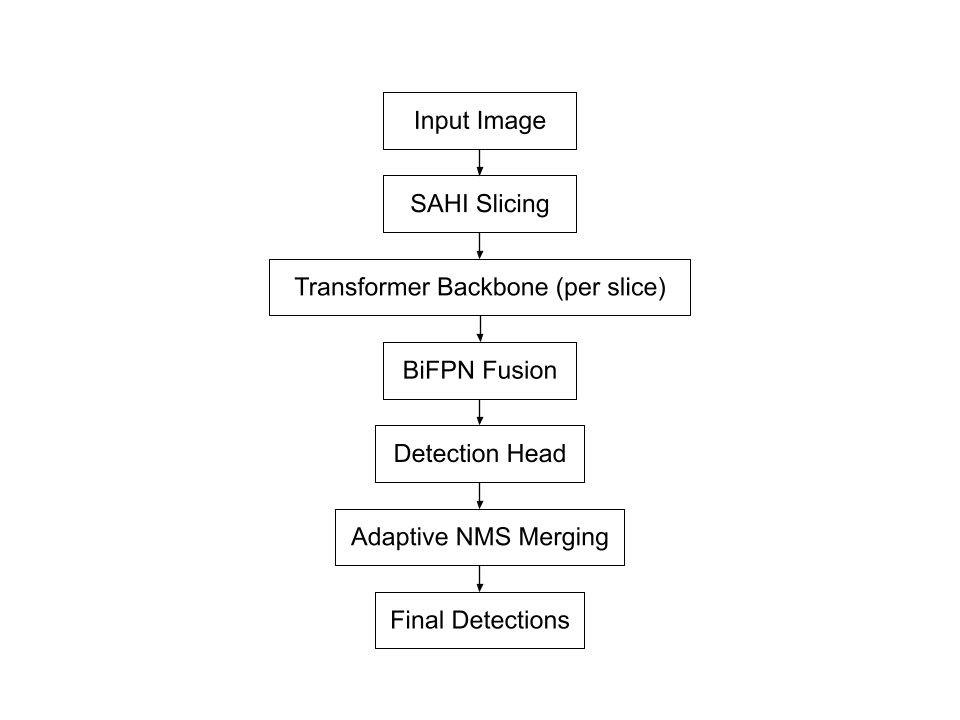
\includegraphics[width=0.9\columnwidth]{pipeline.png}
	\caption{The proposed SAT-Net inference pipeline. A high-resolution image is sliced into overlapping patches. Each patch is processed by our detection model, and the resulting detections are merged using an adaptive NMS to produce the final output.}
	\label{fig:pipeline}
\end{figure}

\subsection{High-Resolution Sliced Inference}

Traditional detectors must downsample large input images (e.g., 2000$\times$1500 pixels) to fit memory constraints (e.g., 640$\times$640). For small objects, which may only be 32$\times$32 pixels or smaller (as defined in our experiments), this aggressive downsampling can reduce them to a single-pixel representation, or erase them entirely.

To combat this, we adopt the core principle of Slicing-Aided Hyper Inference (SAHI)~\cite{aksoy2022slicing}. Instead of downsampling the entire image, we first slice the original high-resolution image into $N$ overlapping patches. Based on our preliminary tests, we selected a patch size of $640 \times 640$ pixels with a $25\%$ overlap between adjacent patches.

This approach ensures that inference is performed on high-resolution regions of the image. A small object that occupied $32 \times 32$ pixels in the original image retains its full pixel fidelity within the $640 \times 640$ slice, allowing the detector's backbone to extract much richer spatial and semantic features.

\subsection{Transformer-based Feature Extraction and Fusion}

While slicing preserves detail, each patch suffers from a lack of global context. A detector processing one slice has no information about the content in other slices. To mitigate this, a highly robust feature extractor is required.

Unlike standard CNNs, which build context through stacked local convolutions, we employ a transformer-based backbone, inspired by models like the Deformable DETR~\cite{zhu2021deformable}. The self-attention mechanism in a transformer is inherently designed to capture global context by modeling long-range dependencies between all feature points. The deformable attention variant specifically allows the model to focus on a sparse set of key sampling points, making it highly effective for localizing small, information-sparse objects.

The features extracted from the transformer backbone are then fed into a Bidirectional Feature Pyramid Network (BiFPN)~\cite{tan2020efficientdet}. A standard FPN~\cite{lin2017focal} passes semantic information down a top-down pathway. A BiFPN adds a second, bottom-up pathway, allowing low-level, high-resolution features to be repeatedly refined with high-level semantic context. This bidirectional flow is critical for small object detection, as it enriches the high-resolution feature maps (where small objects are most visible) with the deep contextual understanding from the network's final layers.

\subsection{Pipeline Integration and Merging}

The complete methodology (Fig.~\ref{fig:pipeline}) integrates these components into a single inference pipeline:
\begin{enumerate}
	\item A high-resolution input image (e.g., from MS COCO or SODA-D) is received.
	\item The image is divided into $N$ overlapping $640 \times 640$ patches.
	\item Each patch is passed independently through our SAT-Net model (Transformer backbone + BiFPN neck + anchor-free detection head).
	\item The bounding box coordinates from each patch's detections are mapped back to the original image's coordinate system.
	\item Due to the $25\%$ patch overlap, a single object may be detected multiple times. To resolve these duplicates, a final Adaptive Non-Maximum Suppression (NMS) is applied to the complete set of global detections.
\end{EXAMPLE}
This pipeline-based approach allows our model to "see" small objects at their original scale, as shown in the "Experiments" section, leading to a significant performance increase over single-pass detectors like RetinaNet and YOLOX.


\end{document}